\subsubsection{\stid{6.02}LLNL ATDM Data \& Viz Projects: ROVER}

%%{\itshape
%%
%%	\begin{enumerate}
%%	\item Rename this file to your project WBS-projectname.tex, for example 2.3.3.01-XSDK4ECP.tex.
%%	\item Complete this template for your project.  Limit your text to two pages, not counting citations.  
%%	\item Please avoid changing the content of main.tex.  
%%	\item Put any references in a .bib file with the same root name, for example 2.3.3.01-XSDK4ECP.bib.
%%	\item Remember to include any image files you reference in your text.
%%    \item The files 2.3.3.01-XSDK4ECP.tex, 2.3.3.01-XSDK4ECP.bib and xSDK-diagram.jpeg are included as examples for your reference.  You can remove them from what you upload.
%%	\end{enumerate}
%%}

\paragraph{Overview} 

ROVER is a generalized ray tracing framework for distributed-memory volume
rendering and simulated radiography \cite{rover-laney} focused on many-core architectures (e.g.,
GPU, CPU, and MIC).  Figure \ref{fig:rover-overview} shows the two use-cases
supported by ROVER. Volume rendering, also known as volume visualization, is a
commonly used scientific visualization algorithm that enables users to
visualize an entire scalar field at once by mapping scalar values to colors and
transparency.  Simulated radiography is a generalization of the volume
rendering algorithm from four color channels (i.e., red, green, blue, and
transparency) to an arbitrary number of channels representing material
opacities in discrete photon energy groups. ROVER leverages VTK-m
\cite{rover-vtkm} for portable performance across many-core architectures. 
\begin{figure}[htb]
	\centering
	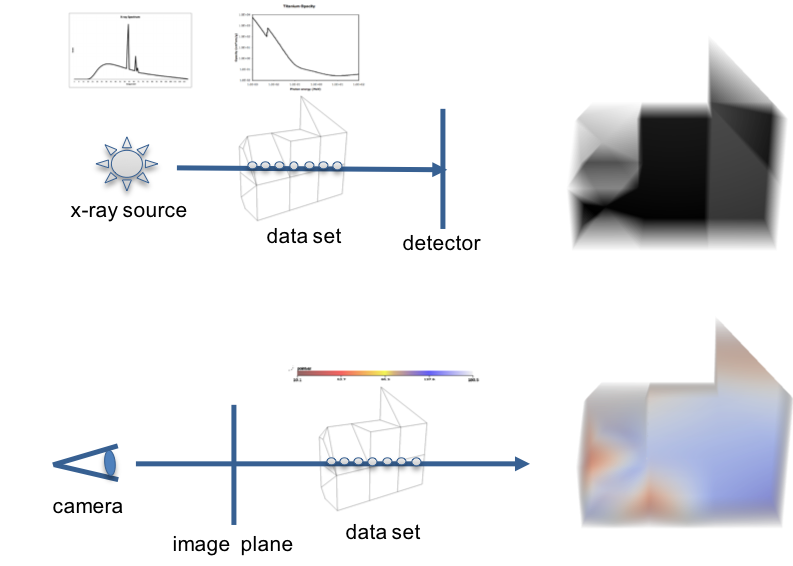
\includegraphics[width=6in]{projects/2.3.6-NNSA/2.3.6.02-LLNL-ATDM/ROVER}
	\caption{\label{fig:rover-overview} (top) Simulated radiography models
the aborption of photons by materials, and requires representation and tracking
of large numbers of photon energies. It also must be highly accurate in terms
of tracking rays through complex meshes. (bottom) volume rendering tracks the
standard RGB and alpha values and is used for scientific visualization where
high performance for user interaction can be important in obtaining good visual
results.} \end{figure}


\paragraph{Key Challenges}
For both volume rendering and simulated radiography, traditional
implementations either do not take advantage of hardware acceleration or
target a single architecture. Existing open source ray-tracing packages do not
support multi-group representations of photon energies.  Furthermore,
raditional implementations of simulated radiography target post-hoc analysis
and are thus ill-suited for use as an in-situ simulated diagnostic. 

ROVER fills a gap in capability: it is designed from the ground-up to be
incorporated into zero-copy in-situ infrastructures, and ROVER uses existing
simulation data distribution to reduce in-situ memory overhead.  It is also
designed to take advantage of modern HPC architectures (CPU, GPU, and MIC),
which maintaining performance even for hundreds of photon energy groups.

\paragraph{Solution Strategy}

First, ROVER is a high-level interface to the low-level ray tracing capability
contained in VTK-m. Second, ROVER provides a custom distributed-memory
compositing capability to combine results from across many nodes into a set of
images or raw floating point values that can be further post-processed. The
development of ROVER required cell intersection kernals, face-to-cell
connectivity generation, and ray integration, all of which have been
contributed directly to VTK-m.  ROVER's distributed memory 
infrastructure handles both ray generation (orthographic and parallel project),
and implements a custom hybrid-parallel compositing implementation for
\textit{n} energy groups, where \textit{n} can be $>100$.

ROVER supports single or double precision integration and includes the ability
to handle self-emmission of photons from mesh elemets. ROVER currently supports
uniform, curvilinear, rectilinear, and unstructured meshes in two and three
dimensions. To enable the high accuracy needed for radiography use-cases,
meshes are traversed using information about the topology (i.e., face-to-face
connectivity) and handling of lost rays is user configurable.

The ROVER code base uses standard MPI (Message Passing Interface) and the
library DIY (Do-It-Yourself-Analysis) to composite the node-level results
produced by VTK-m, a many-core version of the visualization toolkit supported
by ECP (Exascale Computing Project). All libraries used by ROVER are open
source projects, and ROVER does not use any private, vendor specific
programming interfaces or proprietary information. ROVER serves two purposes.

\paragraph{Recent Progress}

The VTK-m ray tracing code was refactored to make it easy to add new
intersection methods (i.e., RZ intersections).  This refactoring enabled the
implementation and testing of RZ intersection routines in VTK-m.  Point
rendering via ray tracing was implemented and tested.  The ROVER project began
working with with the ECP VTK-m team at ORNL on shared milestones ([MS-18/10]
Rendering of topological entities], since there is a great deal of overlap. The
VTK-m team will leverage the refactored code to meet their milestone and in
return they will assist in hardening the refactor.  

\paragraph{Next Steps}
The high level code has been approved for open source release by LLNL to open
source.  After release, we plan to integrate ROVER into VTK-m so it can be
deployed in several downstream projects. These downstream projects are all open
source and include Ascent, VisIt, and ParaView. Ascent is a in situ
infrastructure that is part of the ALPINE ECP project, and Ascent is developed
by LLNL, the University of Oregon, and Kitware Inc. VisIt is a scientific
visualization application developed by LLNL, and ParaView is a scientific
visualization application developed by LANL, Sandia, and Kitware Inc.

